% Chapter 1

\chapter{Introduction} % Write in your own chapter title
\label{Chapter1}
\lhead{Chapter 1. \emph{Introduction}} % Write in your own chapter title to set the page header

Digital video refers to a sequence of images displayed on a screen at a predetermined rate. The process of transferring video content from one medium to another depends on both the duration of the video and the size of the encoded bits. \textbf{Video compression} techniques are commonly utilized to reduce the overall size of the video, which consequently leads to a decrease in the amount of data required for transmission and storage of digital video signals.

The most current video coding standard is known as \textbf{H.264/AVC or MPEG-4 Part-10}. This standard was jointly developed by the \textbf{ITU-T Video Coding Experts Group} and \textbf{ISO/IEC JTC 1 Moving Picture Experts Group}. Compared to typical video coding standards, H.264/AVC provides significantly higher efficiency, capable of reducing bit rate requirements by up to 50$\%$ while maintaining the same level of video quality. It is designed to cover a wide range of video resolutions, from QCIF to HDTV. 
% refrence to ppr J_2008.04

% explain the h.464 profiles and levels 
% ref taken from https://www.rgb.com/h264-profiles#:~:text=Blu%2Dray%20discs.-,H.,Baseline%2C%20Main%2C%20and%20High.
\section{H264 Profiles}
The H.264 family of standards includes various capabilities. These profiles are mainly used to reduce the frame count by implementing motion prediction and temporal compression. The most common ones are:

\begin{itemize}
	\item Baseline Profile
	\item Main Profile
	\item High Profile
\end{itemize}

\subsection{Baseline Profile}
In the realm of video encoding, baseline profiles are commonly employed in applications that require low-power consumption and cost-efficiency. These profiles are capable of achieving an impressive compression ratio of 1000:1, resulting in a streamlet of 1 Gbps being compressed down to approximately 1 Mbps. Baseline profiles utilize a 4:2:0 chrominance sampling method, whereby color information is sampled at half the vertical and horizontal resolution of the black-and-white information. This technique enables the reduction of data without significantly impacting the overall quality of the video.

Furthermore, Universal Variable Length Coding (UVLC) and Context Adaptive Variable Length Coding (CAVLAC) are employed as the primary entropy encoding techniques within this profile. Such encoding methods contribute significantly to the efficient compression of video data, while ensuring that the encoded video stream is in compliance with relevant standards. 

\subsection{Main Profile}
Significant enhancements were made to the Baseline Profile through the introduction of advanced frame prediction algorithms, resulting in the development of the Main Profile. This updated profile is primarily utilized for standard-definition digital TV broadcasts in MPEG-4 format.

However, it should be noted that the Main Profile is not employed in high-definition broadcasts. Rather, alternate profiles are used in such scenarios to ensure optimal video quality and compatibility with relevant standards.

\subsection{High Profile}
Introduced in the year 2004, the High Profile is considered to be the most efficient and powerful profile within the H.264 family. It is primarily utilized in high-definition television applications such as Blu-ray Disc storage and DVB HDTV broadcast services. This profile is capable of achieving an exceptional compression ratio of 2000:1, which is a significant improvement over previous encoding standards. It utilizes an adaptive transform method that allows for the selection of either 4x4 or 8x8 pixel blocks. This enables preservation of video quality while reducing network bandwidth consumption by up to 50 percent.

Furthermore, the application of this compression technique facilitates the compression of a 1 Gbps stream to approximately 512 Kbps, further emphasizing the impressive capabilities of the High Profile.

The overall procedure of H.264 includes various components. The top level block diagram of an H.264 Encoder is shown in Figure \ref{fig:toplevel}.

% figure here ----------------------------
\begin{figure}[htbp]
	\centering
	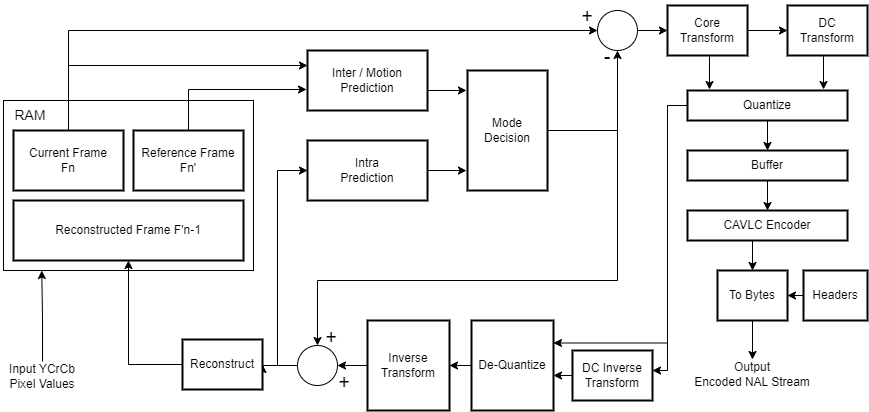
\includegraphics[width = 5in]{./Figures/toplevel.png}
	\rule{35em}{0.5pt}
	\caption{Top Level Diagram for H.264 Encoder}
	\label{fig:toplevel}
\end{figure}

% explain the components briefly
\section{H264 Process}
An H264 encoder has a \textbf{forward path} and a \textbf{reconstruction path}. The forward path uses \textbf{intra} and \textbf{inter predictions} to encode a video frame to create a bit stream. The reconstruction path is used to decode the encoded frame and to reconstruct the decoded frame. Reconstruction path in encoder ensures that both encoder and decoder make use of similar reference frames for inter and intra prediction. This is to avoid encoder-decoder mismatches. 

\subsection{Forward Path}
The input frame is partitioned into \textbf{Macro-Blocks (MB)}. These MB are then encoded in intra or inter mode. This depends on mode decision. The current MB is predicted from reconstructed frame. This predicted MB is generated by intra prediction based on \textbf{spatial redundancy}, and by inter prediction based on \textbf{temporal redundancy}. The mode is chosen based on better quality and bit rate performance of these 2 modes. The Predicted MB is subtracted from current MB to create a \textbf{Residual MB}. Residual data is \textbf{transformed} (4x4 integer transform), then \textbf{quantized}. The obtained coefficient are re-ordered in a \textbf{zig-zag order} which are regarded as \textbf{entropy encoded}. These coefficients along with header information form the \textbf{compressed bit stream}. This stream is forwarded to NAL for storage or transmission. 

\subsection{Reconstruction Path}
This path takes quantized transform coefficients and performs inverse quantization and inverse transform. In this way, reconstructed residual data is generated, but they are not identical to original residual data as quantization is a lossy process. In order to create the reconstructed frame, the reconstructed residual data are added to predicted pixels. 

% refrence material being taken from Richardson book
\section{H264 Major Components}

\subsection{Prediction}
In order to guarantee a high compression ratio in H.264 encoders, prediction is a technique utilized. In prediction, a 16x16 pixel block known as a macroblock from a previous video frame or the present frame is utilized to forecast macroblocks in the current frame. 

There are basically 2 modes for prediction:

\subsection{Intra-Prediction}
Intra prediction is performed without referring to any data outside the current slice i.e prediction from previously coded data in the same slice. It reduces spatial redundancies by exploiting spatial correlation between adjacent blocks in a given picture. There are 3 choices of block size for luma component i.e. 16x16, 8x8 or 4x4. Whereas for chroma component, a single prediction block is generated. Once, the prediction has been made, it is subtracted from current block to make a residual. 
%include diagram

\subsection{Inter-Prediction}
Inter prediction is the process of predicting a block of luma and chroma samples from a picture that has been previously coded and transmitted i.e reference picture. It uses temporal sampling technique. For this, a prediction region is selected, then a prediction block is generated. After that the prediction block is subtracted from original block of samples to form a residual. 
%include diag

\subsubsection{Motion Vector Prediction}
In video coding, motion vectors for neighboring partitions are typically closely related, and so each motion vector can be predicted using previously coded vectors from nearby partitions. A predicted vector is created based on these previous motion vectors, and the difference between the current vector and the predicted vector is encoded and transmitted. The way in which predicted vector is predicted depends on the size of the motion compensation partition and whether there are nearby vectors available for reference.
%include diagg

\subsection{Transform}
Once theresidual data, which essentially comprises a block of residual coefficients, is obtained, it is subjected to the core transform process. This transform is an integer-based 4x4 or 8x8 transform that provides a scaled approximation to the Discrete Cosine Transform (DCT). In certain cases, a portion of the output from this integer transform is subject to further transformation through a DC Transform, referred to as the Hadamard transform. The same residual data can be reconstructed using the DC inverse transform, which is carried out prior to rescaling. Finally, the rescaled coefficients are inverse transformed using a 4x4 or 8x8 inverse integer transform.

\subsection{Quantization}
The transformed coefficients are subjected to quantization using a non-uniform quantizer. In this process, each coefficient is divided by an integer value, which reduces the precision of the coefficient values as determined by the Quantization Parameter (QP). The use of a non-uniform quantizer results in a smaller number of bits being used to represent each coefficient value, which in turn reduces the amount of data required to represent the video. The quantized transform coefficients of a block are typically scanned in a zig-zag pattern, which is a common approach for video coding standards.

\subsection{Entropy Encoding}
In H.264 stream or file encoding, the symbols are coded in a series. The quantized transform coefficients are efficiently transmitted using the Context-Adaptive Variable Length Coding (CAVLC) method. The statistical distribution of the quantized transform coefficients typically shows larger values for low-frequency components that decrease gradually towards the high-frequency part. As a result, the number of nonzero quantized coefficients (N) and their size and position are coded separately. This enables the receiver to reconstruct the original signal more accurately. The coefficients are scanned in a zig-zag pattern, and then quantized to reduce their precision using the quantization parameter (QP). The efficient transmission of quantized transform coefficients in H.264 helps in reducing the size of the compressed video file while maintaining the quality of the video.

% include h.264 syntax briefly
% taken from the richardson book
\section{H264 syntax}
H.264 consists of 2 layers: the \textbf{Network Abstraction Layer (NAL)} and the \textbf{Video Coding Layer (VCL)}. The NAL consists of a series of NAL Units, with \textbf{Sequence Parameter Sets (SPS)} and \textbf{Picture Parameter Sets (PPS)} being the most common units that signal certain control parameters to the decoder. In the VCL, coded video data is communicated in the form of slices.An \textbf{access unit}, which can be a coded frame or field, is made up of one or more slices. Each slice consists of a Slice Header and Slice Data, with the latter being a series of coded \textbf{macro blocks (MB)} and skip macro block indicators signaling that certain macro block positions contain no data.

\begin{itemize}
	\item \textbf{MB type:} I/intra coded, P/inter coded from one reference frame
	\item \textbf{Prediction information:} prediction mode for I macro block, choice reference frame and motion vectors for P macro block
	\item \textbf{Coded Block Pattern CBP:} indicates which luma and chroma blocks contain non zero residual co-efficient
	\item \textbf{Quantization Parameter QP:} for macro blocks with CBP not 0
	\item \textbf{Residual Data:} for blocks containing non-zero residual coefficients
\end{itemize}

The basic H264 syntax can be seen in figure
% draw the digram of layers here

(write something about hardware implementation on FPGA )
In this thesis, we developed an FPGA based H.264 intra and inter frame coder hardware targeting \textbf{High Profile} (see which one to mention, See from wikipedia )

(write about what is happening in the next chapters)